\documentclass{elegantbook}

\definecolor{LightGray}{gray}{0.9}
\newcommand{\CN}{BIOS 7300\\[0.5cm] Survival Data Analysis}
\newcommand{\Ti}{Homework 10}
\newcommand{\Pf}{Dr.\ Tang}
\newcommand{\FN}{Zehao}
\newcommand{\LN}{Wang}
\usepackage[fontsize=14pt]{fontsize}

\usepackage{longtable}

\usepackage{minted}

\usepackage{enumitem}
\renewcommand{\chaptername}{Homework}
\begin{document}
\begin{titlepage}
    \begin{center}    
    
\includegraphics[width=0.6\textwidth]{Tulane.png}\\[1cm]    
    
    \textsc{\Huge \CN}\\[0.5cm]
    \textsc{\large \Pf}\\[1.0cm]
    
    \textsc{\LARGE \Ti}\\[0.5cm]
    \textsc{\large \LN, \FN}\\
    {Master student in Statistics of Math Dept.}
    
    % Author and supervisor
    
    \vfill
    
    % Bottom of the page
    {\Large \emph{\today}}
    
    \end{center}
\end{titlepage}

\thispagestyle{empty}
\tableofcontents
\setcounter{chapter}{9}
\chapter{}

\begin{exercise*}[1]
    Fit the data with the Weibull accelerated failure time model:
    \[S_i(t)=\exp\left(-\lambda\exp(\beta_1Age_i\beta_2 I(Treatment_i=1))^{-\gamma}t^\gamma\right)\]
    where $S_i(t)$ is the survival for the ith subject. Based on this model, answer the following questions.
    \begin{enumerate}[(a)]
        \item Are there significant differences between the two treatment groups? 
        \item Estimate the ratio of median survival times for subjects in the two groups (and the same age).
        \item Estimate the hazards ratio between subjects in the two groups (and the same age). 
        \item Estimate the median survival times for subjects with age=60 in the two groups.
    \end{enumerate}
\end{exercise*}


\begin{solution}
    \begin{minted}[frame=lines,
        framesep=2mm,
        baselinestretch=1.2,
        bgcolor=LightGray,
        fontsize=\footnotesize,
        breaklines=true]{SAS}
DATA HW10; 
    INFILE 
        "Z:\Documents\GitHub\MS-Stat-Tulane\
        Survival_Data_Analysis\HW10\
        Comparison of two treatments for prostatic cancer.dat"
    FIRSTOBS = 2;
    INPUT patient treatment time status age shb size index;
RUN;
PROC LIFEREG DATA=HW10;
    CLASS treatment;
    MODEL time*status(0) = age treatment / DIST=weibull;
run;
    \end{minted}
    \begin{figure}[H]
        \centering
        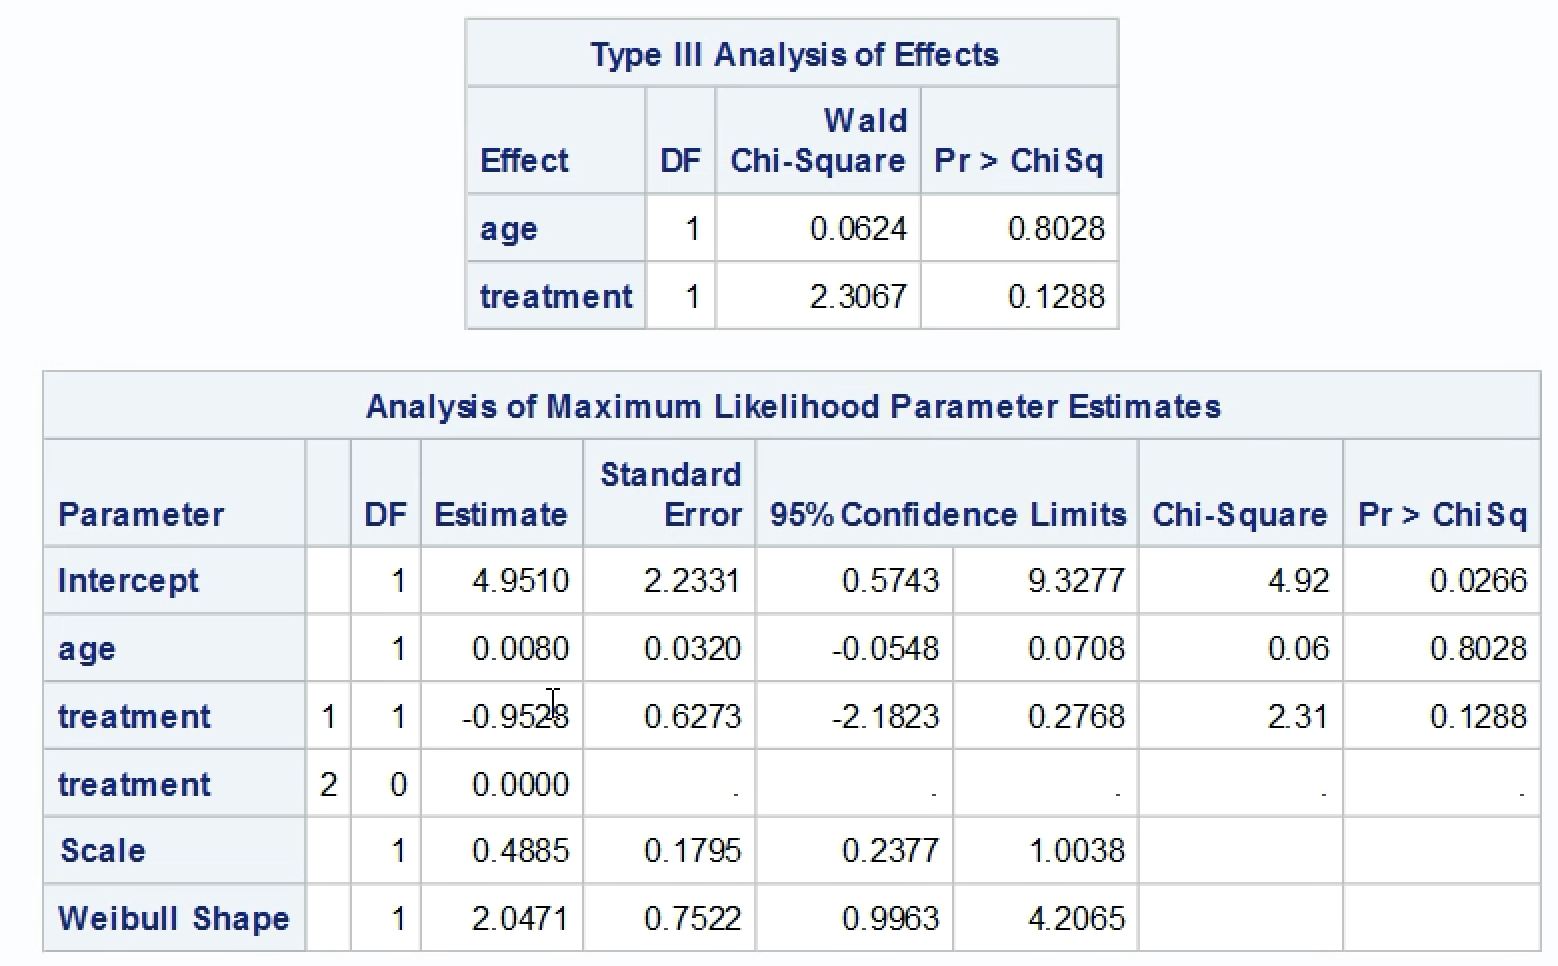
\includegraphics[width=0.7\textwidth]{HW10_1.png}
    \end{figure}
\begin{enumerate}[(a)]
    \item No, we can see that the p-value for treatment is $0.1288>0.05$. 
    \item The ratio of median survival times for subjects in the two groups (and the same age) is 
    \[\frac{t_{50}(treatment=1)}{t_{50}(treatment=2)}=\exp(-0.9528)=0.386. \]
    \item \begin{align*}
        &HR(treatment\ 1\ V.S.\ treatment\ 2)\\
        =&\exp(0.9528/\sigma)=\exp(0.9528/0.4885)=7.032. 
    \end{align*}
    \item Treatment 1:
    \[ t_{50} = (-\log0.5)^{0.4885} \exp( 4.951 + 0.008 \times 60 - 0.9528 )= 73.638. \]
    Treatment 2: 
    \[t_{50} = (-\log0.5)^{0.4885} \exp(4.951 + 0.008 \times 60) = 190.940. \]
\end{enumerate}
\end{solution}

\begin{exercise*}[2]
    Fit the data with the log-logistic regression model
    \[\log t=\beta_0+\beta_1 Age +\beta_2 I(Treatment=1)+\sigma\varepsilon\]
    where $\varepsilon$ follows the standard logistic distribution. Based on this model, answer the following questions. 
    \begin{enumerate}[(a)]
        \item Are there significant differences between the two groups? 
        \item Interpret the coefficients $\beta_1$ and $\beta_2$. 
        \item Estimate the median survival times for subjects with $age=60$ in the two groups. 
        \item Estimate the hazard ratio for subjects with $age=60$ in the two groups at time $t = 70$.
    \end{enumerate}
\end{exercise*}


\begin{solution}
    \begin{minted}[frame=lines,
        framesep=2mm,
        baselinestretch=1.2,
        bgcolor=LightGray,
        fontsize=\footnotesize,
        breaklines=true]{SAS}
PROC LIFEREG DATA=HW10;
    CLASS treatment;
    MODEL time*status(0) = age treatment / DIST=llogistic;
RUN;
    \end{minted}
    \begin{figure}[H]
        \centering
        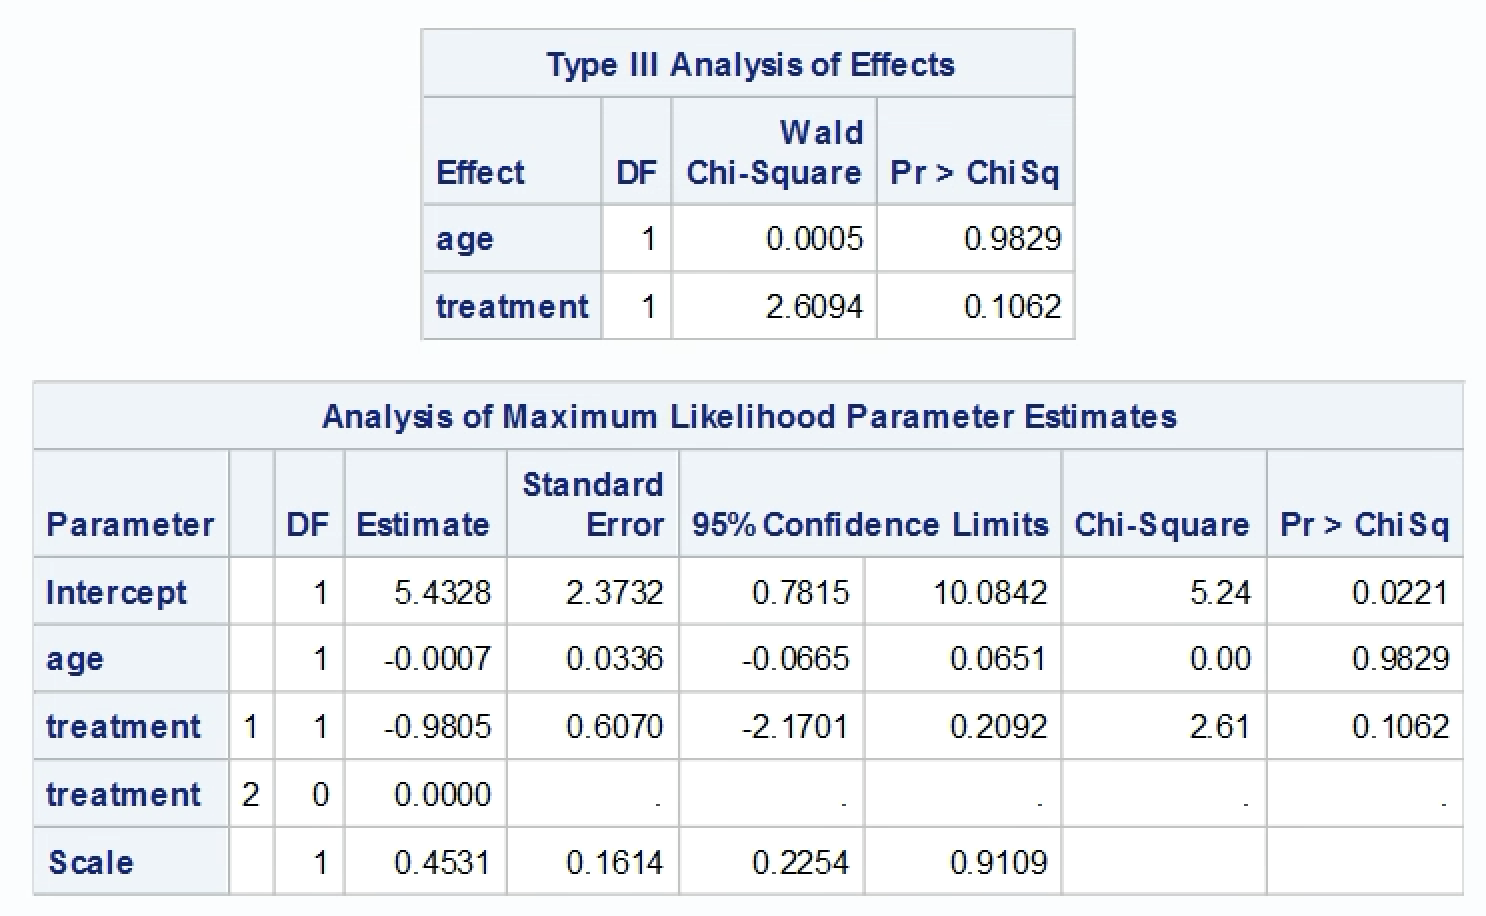
\includegraphics[width=0.7\textwidth]{HW10_2.png}
    \end{figure}
\begin{enumerate}[(a)]
    \item No, we can see that the p-value for treatment is $0.1062>0.05$. 
    \item $\beta_1=-0.0007$: if age increases one unit, $\log(time)$ decreases 0.0007; 
    
    $\beta_2=-0.9805$: if treatment is 1, $\log(time)$ decreases 0.9805 compared to treatment 2; 
    \item Treatment 1:
    \[ t_{50} = \exp( 5.4328 - 0.0007 \times 60 - 0.9805 )= 82.294. \]
    Treatment 2: 
    \[t_{50} = \exp(5.4328 - 0.0007 \times 60) = 219.379. \]
    \item \[HR(T1\ V.S.\ T2;\ Age=60,\ t=70)=\exp(-\beta_2/\sigma)=8.7057. \]
\end{enumerate}
\end{solution}

\begin{exercise*}[3]
    Fit the data with the linear regression model
    \[t=\beta_0+\beta_1 Age +\beta_2 I(Treatment=1)+\varepsilon\]
    where $\varepsilon$ follows a normal distribution. Based on this model, answer the following questions. 
    \begin{enumerate}[(a)]
        \item Are there significant differences between the two groups?
        \item Interpret the coefficients $\beta_1$ and $\beta_2$. 
        \item Estimate the median survival times for subjects with $age=60$ in the two groups. 
        \item Compared with the models in Problems 1 and 2, which model do you think fits
        the data the best?
    \end{enumerate}
\end{exercise*}


\begin{solution}
    \begin{minted}[frame=lines,
        framesep=2mm,
        baselinestretch=1.2,
        bgcolor=LightGray,
        fontsize=\footnotesize,
        breaklines=true]{SAS}
PROC LIFEREG DATA=HW10;
    CLASS treatment;
    MODEL time*status(0) = age treatment / D=NORMAL;
RUN;
    \end{minted}
    \begin{figure}[H]
        \centering
        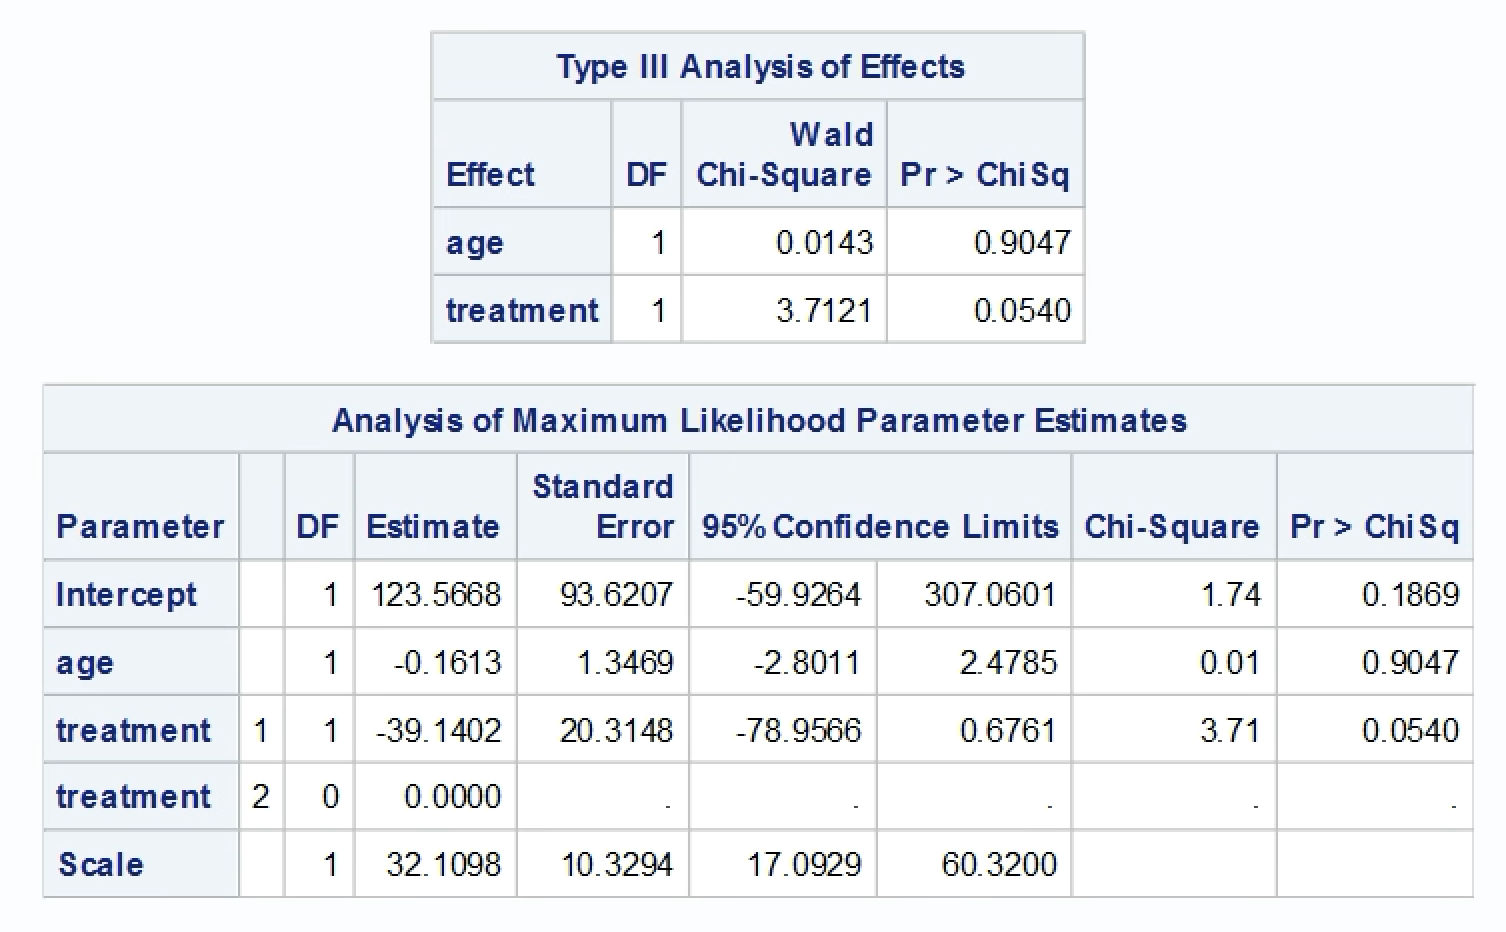
\includegraphics[width=0.7\textwidth]{HW10_3.png}
    \end{figure}
\begin{enumerate}[(a)]
    \item No, we can see that the p-value for treatment is $0.0540>0.05$. 
    \item $\beta_1=-0.1613$: if age increases one unit, survival time decreases $0.1613$; 
    
    $\beta_2=-39.1402$: if treatment is 1, survival time decreases 39.1402 compared to treatment 2; 
    \item Treatment 1:
    \[ t_{50} = 123.5688 - 0.1613 \times 60 - 39.1402 = 74.7506. \]
    Treatment 2: 
    \[t_{50} = 123.5688 - 0.1613 \times 60 = 113.8908. \]
    \item The AIC for these three models are as follows: 
    \begin{figure}[H]
        \centering
        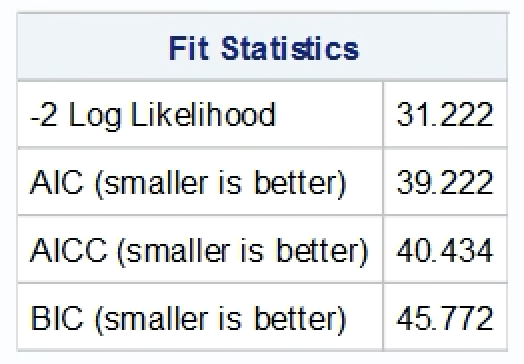
\includegraphics[width=0.3\textwidth]{HW10_3_1.png}\\
        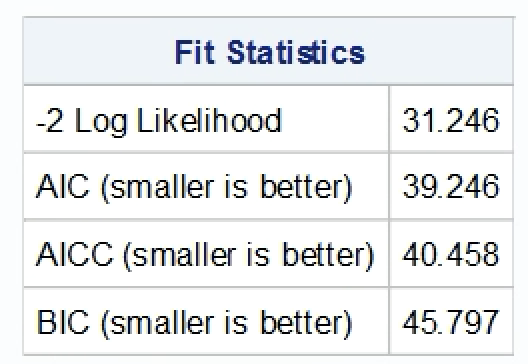
\includegraphics[width=0.3\textwidth]{HW10_3_2.png}\\
        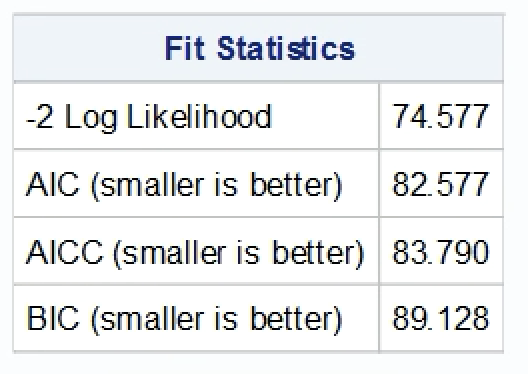
\includegraphics[width=0.3\textwidth]{HW10_3_3.png}
    \end{figure}
    The model with the smallest AIC is the weibull model, so I think the weibull model fits the data the best.
\end{enumerate}
\end{solution}



\end{document}



